\section{Fine-tuning for ASR with Wav2Vec 2.0}

\begin{frame}{}
    \LARGE \textbf{Fine-tuning for ASR with Wav2Vec 2.0}
\end{frame}

\begin{frame}{Fine-tuning Overview}
    \begin{itemize}
        \item \textbf{Self-Supervised Learning (SSL):} Pre-train Wav2Vec 2.0 on large unlabeled audio.
        \item \textbf{Fine-tuning:} Use small labeled dataset for ASR.
        \item \textbf{Loss Function:} Connectionist Temporal Classification (CTC) Loss.
        \item \textbf{Goal:} Map audio features to text transcriptions.
    \end{itemize}
\end{frame}

\begin{frame}[allowframebreaks]{Fine-tuning Results}
    \begin{itemize}
        \item \textbf{Small labeled data:} Only 10 minutes of transcribed speech.
        \item \textbf{Performance:} Word Error Rate (WER) 4.8\% (test-clean) / 8.2\% (test-other).
        \item \textbf{Read the small print.} That headline number needs all three of:
        \begin{itemize}
            \item the \textsc{Large} model ($\sim$317M parameters),
            \item pre-training on 53k hours of unlabeled LibriVox audio (LV-60k),
            \item a Transformer language model at decoding time.
        \end{itemize}
        Swap the LM for a 4-gram and the same model gives 6.6\% / 10.3\%; decode with no LM at all and it is around 40\%. The \textsc{Base} model at 10 minutes gives 6.9\% / 12.9\%.
        \item \textbf{Efficient:} High accuracy with minimal \emph{supervision}, not with minimal compute or data.
    \end{itemize}
\framebreak
    \begin{center}
        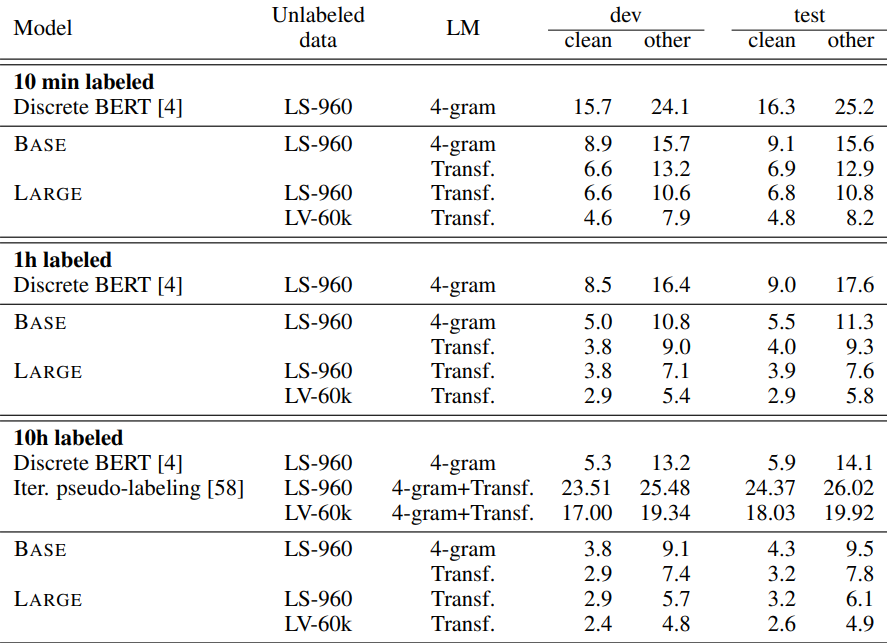
\includegraphics[width=\textwidth,height=0.82\textheight,keepaspectratio]{images/audio-nlp/wav2vec2-wer-results.png}
    \end{center}
    \vspace{-0.5em}
    {\scriptsize Source: Baevski et al., ``wav2vec 2.0'', NeurIPS 2020, Table~1 (extract).}
\end{frame}

\begin{frame}[fragile]{PyTorch Fine-tuning Example}
    \textbf{Wav2Vec 2.0 + CTC Loss (PyTorch)}
    \begin{lstlisting}[language=Python]
import torch
import torchaudio
from transformers import Wav2Vec2ForCTC, Wav2Vec2Processor

processor = Wav2Vec2Processor.from_pretrained("facebook/wav2vec2-base-960h")
model = Wav2Vec2ForCTC.from_pretrained("facebook/wav2vec2-base-960h")

input_audio, _ = torchaudio.load("audio.wav")
inputs = processor(input_audio.squeeze(), sampling_rate=16000, return_tensors="pt")
with torch.no_grad():
    logits = model(**inputs).logits
pred_ids = torch.argmax(logits, dim=-1)
transcription = processor.decode(pred_ids[0])
print(transcription)
    \end{lstlisting}
\end{frame}

\begin{frame}{Decoding: Beam Search / Viterbi}
    \begin{columns}[T,onlytextwidth]
        \begin{column}{0.36\textwidth}
            \begin{itemize}
                \item \textbf{CTC Decoding:}
                \begin{itemize}
                    \setlength{\itemsep}{1em}
                    \item Greedy decoding: Select most probable token at each timestep.
                    \item Beam search: Explore multiple hypotheses for better accuracy.
                    \item Viterbi algorithm: Find most likely sequence.
                \end{itemize}
                \item \textbf{Equation:}
                \[
                    \hat{y} = \arg\max_{y} P(y|x)
                \]
            \end{itemize}
        \end{column}
        \begin{column}{0.6\textwidth}
            \begin{center}
                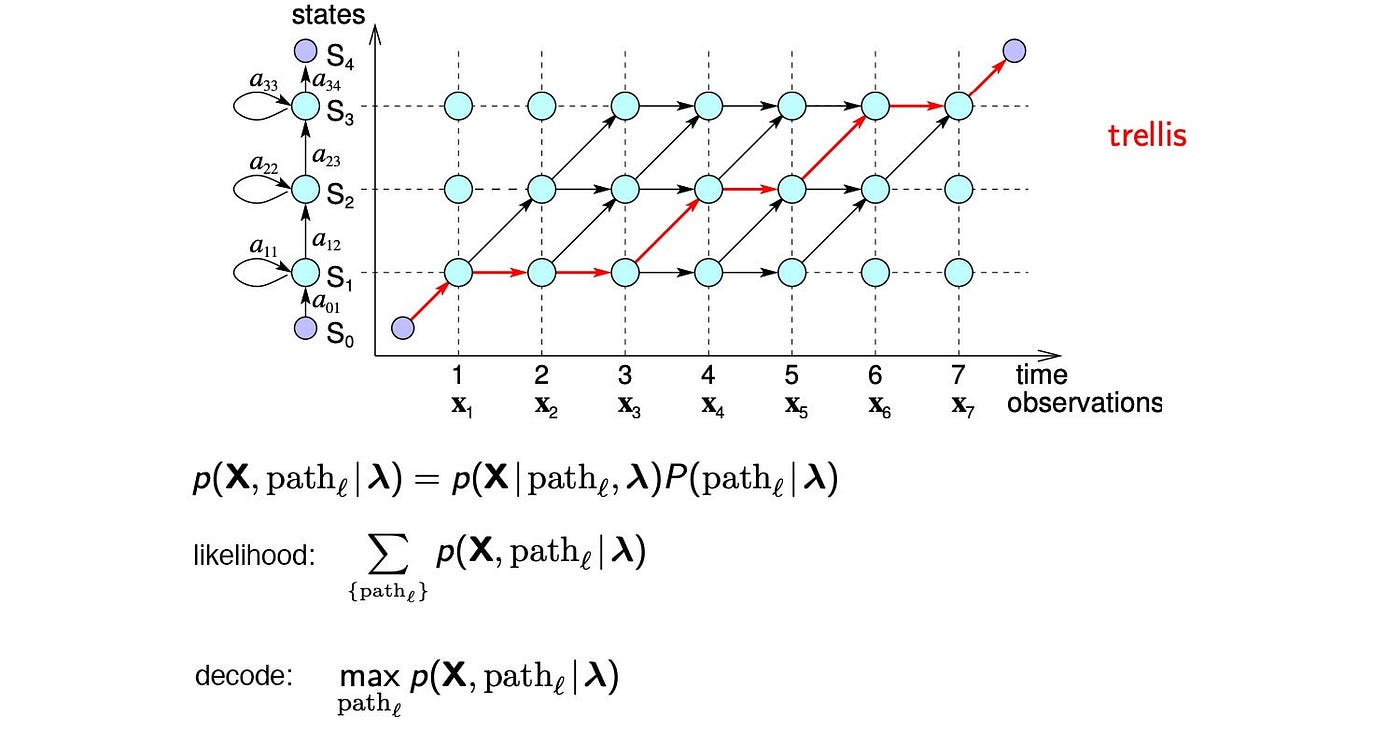
\includegraphics[width=\textwidth]{images/audio-nlp/ctc-decoding.png}\\
                {\scriptsize The same sum-over-paths (likelihood) vs.\ max-over-paths (Viterbi) choice, drawn on an HMM trellis.\\
                Source: H.~Shimodaira and S.~Renals, ``Hidden Markov Models and Gaussian Mixture Models,'' Automatic Speech Recognition Lectures 4--5, University of Edinburgh.}
            \end{center}
        \end{column}
    \end{columns}
\end{frame}